\documentclass[10pt]{standalone}
\usepackage{amsmath}
\usepackage{amssymb}
\usepackage{pgf,tikz}
\usepackage{mathrsfs}
\usetikzlibrary{arrows,calc,positioning,shapes.symbols,shapes.geometric}
\pagestyle{empty}

\begin{document}
  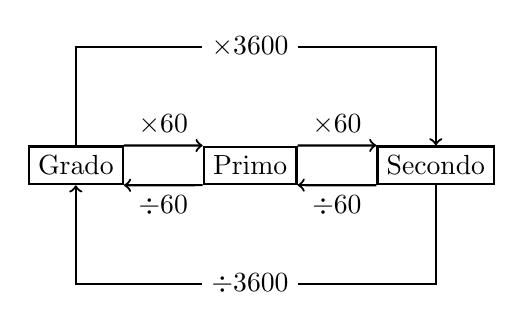
\begin{tikzpicture}
  \tikzset{every picture/.style={scale=0.3,every picture/.style={}}}
  \tikzset{main base/.style={draw,thick,text centered, }, }
  \tikzset{main node/.style={rectangle, draw,main base}, }
  \tikzset{main node2/.style={main node,
  		text width=7em, minimum height=3em}, }
  \tikzset{main verb/.style={minimum size=2.5cm}, }
  \tikzset{linea/.style={-triangle 90,thick,draw}}
  \tikzstyle{etichetta}=[midway]
  %\tikzset{linea/.style={-triangle 90,thick,draw}}
  \tikzset{linea2/.style={-triangle 90,draw}}
  \tikzset{primo/.style={circle,draw,inner sep=0pt,minimum size=1pt,thick}, }
    \node[main node] (g) {Grado};
    \node[main node] (m) [right =of g]  {Primo};
    \node[main node] (s) [right=of m]  {Secondo};
    \node(ptop) [below=of m]{$\div3600$};
    \node(pdown) [above=of m]{$\times3600$};
    \draw[linea,->] (g.north east)--(m.north west)node[etichetta,above]{$\times 60$};
    \draw[linea,->] (m.north east)--(s.north west)node[etichetta,above]{$\times 60$};
    \draw[linea,<-] (g.south east)--(m.south west)node[etichetta,below]{$\div 60$};
    \draw[linea,<-] (m.south east)--(s.south west)node[etichetta,below]{$\div 60$};
    \draw[linea,->](g)|-(pdown)-| (s);
    \draw[linea,->](s)|-(ptop)-| (g);
\end{tikzpicture}
\end{document}